% !TEX root =../LibroTipoETSI.tex
\chapter{Protocolo MQTT y STOMP}\LABCHAP{MQTT}
\pagestyle{esitscCD}

\section{MQTT}

\texttt{MQTT} es un protocolo cliente/servidor que permite roles de publicador/suscriptor.
Es ligero, abierto, simple y diseñado para ser fácil de implementar en el cliente.
Estas características lo hacen ideal para su uso en múltiples situaciones, como por ejemplo,
entornos donde la memoria y el ancho de banda son limitados, como la comunicación M2M
(\emph{Machine to machine}) o para dispositivos en el Internet de las Cosas.

Es un protocolo binario ligero que, en comparación con \texttt{HTTP}, tiene una
mínima sobrecarga en cuanto a cabeceras para hacer más eficiente el tampaño de los
paquetes.
\texttt{MQTT} es muy fácil de implementar en el cliente. Esto encaja perfectamente
en sistemas integrados con recursos limitados, de hecho,
esto es uno de los objetivos que se buscaban cuando \texttt{MQTT} se creó.

\subsection{El patrón publicador/suscriptor}

\begin{figure}[htbp]
\centering
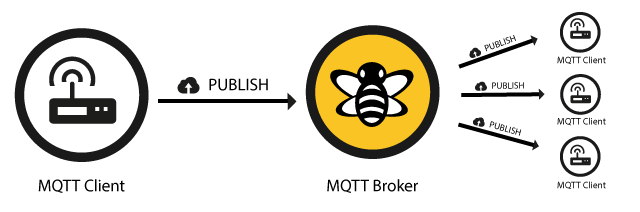
\includegraphics[width=\linewidth]{04-mqtt/figuras/fig001}
\caption{Patrón publicador/suscriptor}
\label{fig:figura1}
\end{figure}

El patrón publicador/suscriptor es una alternativa al sistema tradicional de
cliente/servidor, donde un cliente se comunica directamente con un destino.
Sin embargo, el patrón \texttt{pub/sub} desacopla al cliente que están enviando
un mensaje (publicador) de otro cliente o más clientes que reciben mensajes
(suscriptor). Esto quiere decir que publicador y suscriptor no son conscientes
de la existencia del otro. Existe un tercer componente llamado \emph{broker} que
es conocido tanto por el publicador como el suscriptor que es el encargado de
filtrar los mensajes que llegan y distribuirlos correctamente.

As already mentioned the main aspect in pub/sub is the decoupling of publisher and receiver, which can be differentiated in more dimensions:
Como ya hemos mencionado, el pricipal aspecto del patrón publicador/suscriptor
es el desacople en las siguientes dimensiones:

\begin{itemize}\itemsep1pt \parskip0pt \parsep0pt
\item Espacio desacoplado: Publicador y suscriptor no tiene porqué saber el uno del otro (IP, puerto, etc.).
\item Tiempo desacoplado: Publicador y suscriptor no tienen porqué estar en ejecución al mismo tiempo.
\item Sincronización desacoplada: Las operaciones de los dos componentes no se detienen durante envío o recepción.
\end{itemize}

En resumen, el patrón publicador/suscriptor desacopla el publicador o receptor de
un mensaje y a través de los filtros para los mensajes se puede elegir qué clientes
reciben qué mensajes.

\subsection{Escalabilidad}

El patrón publicador/suscriptor ofrece mejor escalabilidad que el patrón clásico
de cliente/servidor. Esto se debe a que las operaciones en el broker pueden ser
altamente paralelizadas. También es común el cacheo de mensajes y el enrutado
inteligente. Sin embargo, es un reto el escalar a millones de conexiones, esto
puede conseguirse mediante el uso de clústeres de \emph{brokers} para distribuir
la carga entre múltiples servidores.

\subsection{Filtrado de mensajes}

El filtrado de mensajes es el encargado de que sólamente los mensajes sean
recibidos por los clientes que deben. Tenemos varias opciones de filtrado de
mensajes:

\begin{itemize}\itemsep1pt \parskip0pt \parsep0pt
\item Filtrado basado en \texttt{topic}: El \texttt{topic} puede ser parte de cada mensaje. Cada
cliente recibe sólamente mensajes del \texttt{topic} en el que está interesado. Los topics
generalmente son cadenas de texto organizadas de forma jerárquica, por lo que se puede
filtrar en función de una expresión.
\item Filtrado basado en contenido: El filtrado se basa en el contenido específico
del mensaje. Una gran desventaja de este método es que el contenido del mensaje
debe ser conocido por el \emph{broker}, cosa que no siempre ocurre, por ejemplo,
cuando el contenido va cifrado.
\item Filtrado por tipo: En lenguajes orientados a objetos es típico filtrar en
base a un tipo o clase del mensaje o evento. En este caso el suscriptor podría
recibir todos los mensajes de un tipo o subtipo.
\end{itemize}

En el caso de \texttt{MQTT} se utiliza el filtrado por \texttt{topic} así que cada
mensaje contiene un \texttt{topic}, el cual es procesado por el \texttt{broker}
para entregarlo a los clientes que se han suscrito a él.

\texttt{MQTT} tiene múltiples niveles de calidad de servicio (QoS). Se puede
conseguir fácilmente que un mensaje sea entregado del cliente al \emph{broker} o
del \emph{broker} al cliente. Sin embargo, existe la posibilidad de que nadie
se suscriba a un \texttt{topic} en particular, en este caso depende el \emph{broker}
cómo se debe manejar la situación.

\subsection{Diferencias con un sitema de colas}

Existe confusión debido a su nombre en cuanto a sí es un protocolo de colas.
Su nombre proviene de \emph{MQseries}, un producto de \emph{IBM} y no de \emph{Message Queue}.
Independientemente del nombre, existen diferencias entre \texttt{MQTT} y un
sistema de colas:

\begin{itemize}\itemsep1pt \parskip0pt \parsep0pt
\item Un sistema de colas almacena un mensaje hasta que se consume: En un sistema
clásico los mensajes se almacenan hasta que son tomados por un cliente (consumidor),
esto en \texttt{MQTT} no ocurre ya que puede haber cero clientes suscritos a un
topic y el mensaje es descartado.
\item Un mensaje sólo es consumido por un cliente: Otra gran diferencia es el hecho
de que en un sistema tradicional de cola de mensajes, los mensajes son consumidos
por un único consumidor así la carga se puede distribuir entre múltiples procesos.
En \texttt{MQTT} esto suele ser al contrario, todos los suscriptores reciben el
mensaje si se han suscrito al \texttt{topic}.
\item Las colas tienen nombres y deben crearse de forma explícita: Una cola es
menos flexible que un \emph{topic}, antes de usar una cola debe declarase
explícitamente y sólo entonces se pueden consumir los mensajes. En \texttt{MQTT}
los \emph{topics} son extremadamente flexibles y son creados en el momento.
\end{itemize}
